\section{Contexto histórico e motivação}

%http://heroicrelics.org/info/v-2/v-2-cut-away.html
%https://v2rockethistory.com/?s=jet+vane

A tecnologia de empuxo vetorial (ou TVC, do inglês \textit{thrust vector control}) é chave para o setor aeroespacial, pois permite aproveitar o empuxo gerado pelo motor-foguete para aplicar um comando de atitude ao veículo. É uma tecnologia desenvolvida desde os primórdios da tecnologia de foguetes, com o míssil V2 sendo um marco notável no histórico do empuxo vetorial e dos foguetes. Este sistema, exibido na figura~\ref{fig:tvc_systems_jet_vanes}, utilizava lâminas de grafite (\textit{jet vanes}) inseridas na exaustão do motor principal para direcionar o escoamento de gases e produzir uma força lateral capaz de direcionar o míssil.

\begin{figure}
    \centering
    \begin{subfigure}{.49\textwidth}
        \centering
        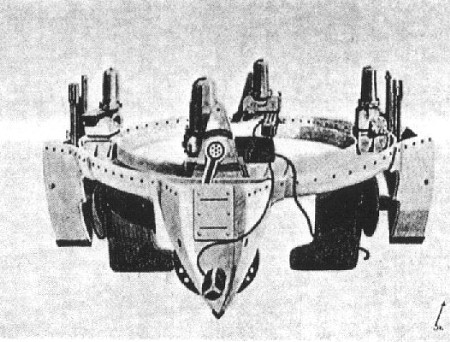
\includegraphics[width=.9\textwidth]{img/v2jetvanes.jpg}
        \caption{Sistema de \textit{jet vanes} do míssil V2~\cite{V2jetvanes}.}\label{fig:tvc_systems_jet_vanes}
    \end{subfigure}
    \hfill
    \begin{subfigure}{.49\textwidth}
        \centering
        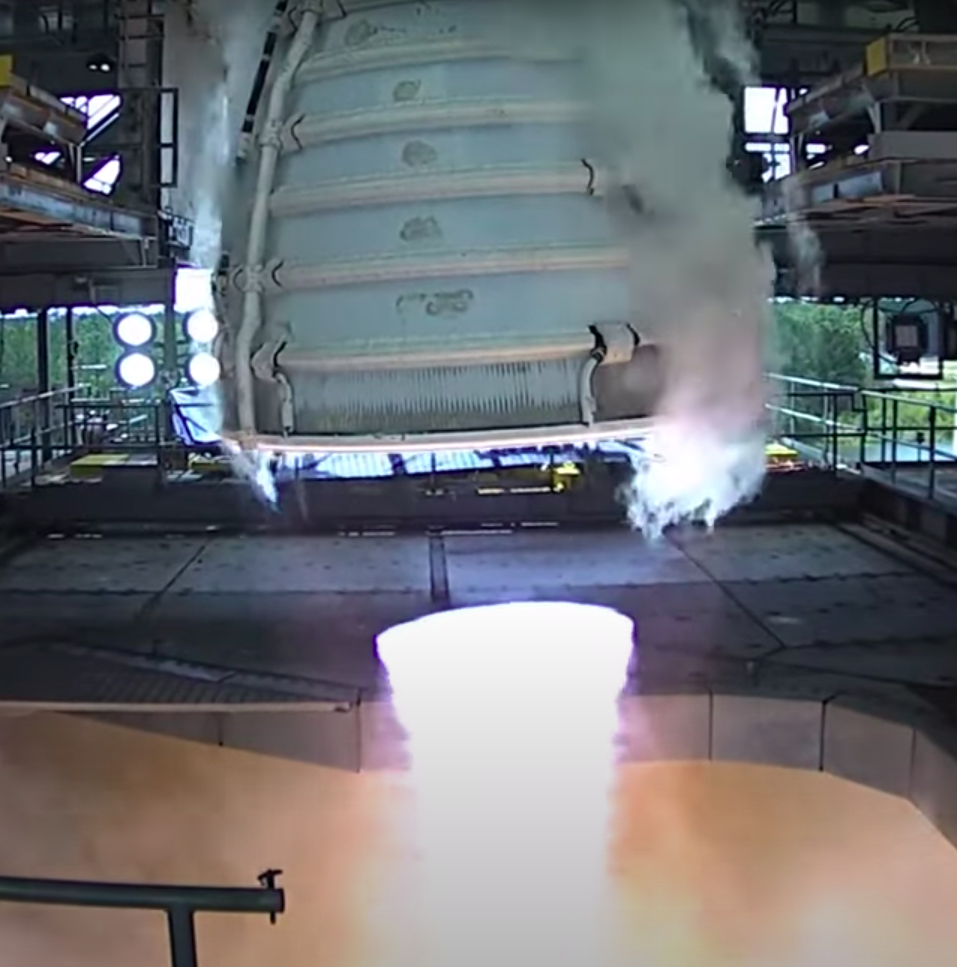
\includegraphics[width=.9\textwidth]{img/engine_gimbal.png}
        \caption{Sistema de \textit{gimbal} do motor RS-25 do foguete Artemis~\cite{RS25Gimbal}.}\label{fig:tvc_systems_gimbal}
    \end{subfigure}
    \caption{Exemplos de sistemas com empuxo vetorial.}
\end{figure}

Outros sistemas de empuxo vetorial foram desenvolvidos após a Segunda Guerra Mundial, tanto para aplicações militares como para lançadores de satélites, cada uma com seus \textit{trade-offs} de engenharia. Uma alternativa de alto desempenho e alta complexidade mecânica muito comum atualmente é a articulação esférica, ou \textit{gimbal}, da tubeira do motor. Um sistema \textit{gimbal}, do motor RS-25 desenvolvido para o ônibus espacial e reaproveitado para o programa Artemis, é exibido em ação na figura~\ref{fig:tvc_systems_gimbal}.

Os sistemas de empuxo vetorial são fundamentais para a estabilidade e para o seguimento de trajetória dos foguetes. Defeitos de manufatura podem introduzir desalinhamentos angulares e lineares de empuxo, que devem ser compensados pelo sistema de controle de empuxo vetorial. Também são fundamentais para o controle dos veículos em baixas velocidades, regime no qual aletas fornecem pouca ou nenhuma autoridade sobre o veículo, permitindo que se elimine a necessidade de trilhos de lançamento. Naturalmente, também funcionam no vácuo espacial. Este trabalho busca, portanto, iniciar uma linha de pesquisa brasileira sobre o assunto.

\section{Objetivos}

Este trabalho buscou desenvolver motor foguete a gás frio de pequena escala (2--5N), um sistema de empuxo vetorial baseado em \textit{jet vane} para direcionamento do empuxo em um plano, e a caracterização empírica das forças geradas pelo sistema, bem como as dificuldades identificadas para o desenvolvimento futuro do tema.

\section{Introdução Teórica}\label{sec:intro}
A propulsão de motores-foguete é baseada na força de reação gerada pela aceleração de uma massa em um sentido oposto ao sentido desejado da força propulsiva. Tecnologicamente, este conceito é implementado com o uso de escoamentos de fluidos compressíveis, acelerados por diferenças de pressão presentes no sistema. Do ponto de vista da engenharia aeroespacial, faz-se necessário conhecer algumas métricas de eficiência que possam ser aplicadas em um projeto. Assim, a propulsão é uma área derivada da mecânica, termodinâmica e engenharia.

No vácuo, força propulsiva, ou empuxo, é uma função do fluxo mássico do sistema, da velocidade de ejeção de propelente (derivada diretamente da segunda lei de Newton). Para sistemas propulsivos em uma atmosfera, deve ser adicionado um termo corretivo referente à diferença de pressão entre a atmosfera e o escoamento ejetado. Assim, o empuxo pode ser dado, em primeira aproximação, por~\cite{Sutton}:
\begin{equation}
    \label{eq:thrust_basic}
    F = \dot{m} v_2 + (p_2 - p_3) A_2
\end{equation}

onde \(F\) é a força propulsiva, \(\dot{m}\) é o fluxo mássico de propelente, \(v_2\) é a velocidade de exaustão do propelente, relativa ao veículo, \(p_2\) é a pressão local na saída da tubeira, \(A_2\) é a área de saída da tubeira e \(p_3\) é a pressão ambiente. Observa-se que a equação~\ref{eq:thrust_basic} assume valores médios para a seção da tubeira. Também, ressalta-se que os índices 2 e 3 referem-se à saída da tubeira e ao ambiente, respectivamente. O índice 1 será usado para referências à câmara.

A razão de expansão é um parâmetro geométrico de um sistema propulsivo, dado por
\begin{equation}
    \label{eq:exp_ratio}
    \varepsilon = \frac{A_e}{A_t}
\end{equation}

onde \(A_e\) é a área da saída da tubeira e \(A_t\) é a área da garganta. Após a garganta, o escoamento está supersônico, e deverá ser acelerado por um aumento da área da seção transversal da tubeira. Assim, a razão de expansão influencia diretamente a velocidade de saída do propelente, descrevendo quanta energia interna (pressão e temperatura) do propelente foi convertida em energia cinética. Razões de expansão maiores implicam em maiores velocidades de saída \(v_2\). No entanto, para motores que operam em uma atmosfera, deve-se atentar também para o fato de que \(p_2\) depende da razão de expansão. Se a razão de expansão for grande demais, haverá uma grande perda de empuxo devido ao segundo termo da equação~\ref{eq:thrust_basic} e, em casos mais graves, descolamento do fluxo e vibrações estruturais intensas. Assim, busca-se otimizar a razão de expansão para uma condição específica.

Um parâmetro de desempenho usado para comparar a eficiência mássica do sistema propulsivo é o impulso específico. Ele mede o impulso imprimido ao veículo por peso de propelente ou, analogamente (supondo regime estacionário), a força gerada por vazão de peso de propelente~\cite{Sutton}:
\begin{equation}
    \label{eq:Isp}
    I_{\text{sp}} = \frac{\int^T_0 F dt}{g_0 \int^T_0 \dot{m}dt} = \frac{F}{g_0 \dot{m}}
\end{equation}

onde \(g_0=9,81m/s^2\). Este fator \(g_0\), a gravidade padrão, foi introduzido para permitir que a unidade do impulso específico seja \(s\), permitindo a fácil comunicação de valores de impulso específico entre instituições que usam o sistema métrico e o sistema imperial. Assim, sistemas propulsivos muito energéticos terão, de modo geral, impulso específico alto, pois conseguem imprimir altas velocidades à massa de reação. Inversamente, sistemas pouco energéticos, como os de gás frio, terão impulsos específicos baixos.

Outro parâmetro útil é o coeficiente de empuxo \(C_F\). Ele mede a amplificação de empuxo advinda da expansão do fluxo supersônico na tubeira do foguete. Ou seja, ele mede a razão entre o empuxo real do sistema e a força que seria obtida aplicando-se a pressão de câmara na área da garganta~\cite{Sutton}:
\begin{equation}
    \label{eq:C_F}
    C_F = \frac{F}{p_1 A_t}
\end{equation}

Se o coeficiente de empuxo mede a eficiência da tubeira, a velocidade característica \(c^*\) mede a eficiência do conjunto câmara e propelente. A velocidade característica é dada por~\cite{Sutton}:
\begin{equation}
    \label{eq:cstar}
    c^* = \frac{p_1 A_t}{\dot{m}}
\end{equation}

A partir das equações~\ref{eq:C_F} e~\ref{eq:cstar} é possível deduzir uma relação muito útil para projeto, que permite o cálculo fácil da vazão mássica necessária:
\begin{equation}
    \label{eq:mdot}
    \dot{m} = \frac{F}{c^* C_F}
\end{equation}

As relações dadas anteriormente assumem que o escoamento está estagnado na câmara de empuxo. Na prática, buscam-se razões \(\frac{A_c}{A_t} \gg 1\) para satisfazer esta hipótese. A literatura recomenda valores mínimos de 4 ou 6~\cite{Sutton}.

%https://software.nasa.gov/software/LEW-17687-1
%https://rocketcea.readthedocs.io/en/latest/
A termodinâmica é capaz de fornecer expressões analíticas para todas as grandezas apresentadas aqui, supondo-se gás perfeito, ausência de reação química e escoamento quasi-unidimensional. No entanto, para uma análise química e termodinâmica mais precisa, busca-se o software CEA NASA, que calcula dos parâmetros propulsivos a partir de certas condições de operação e entradas termodinâmicas do propelente. Com este software, é possível calcular os valores de \(C_F\) e \(c^*\) para um sistema propulsivo com hipóteses menos rígidas que as exigidas pela termodinâmica supersônica. 